
\subsection{Results}

\subsubsection{Crop health survey data}

Prior to using the crop health survey data to construct networks, some exploratory plots of the data are constructed and examined. The figure shows the distribution of the data. A total of 415 farmers' fields was surveyed in Tamil Nadu, India (TMN); West Java; Indonesia (WJV), Laguna, Philippines (LAG); Suphanburi, Thailand (SPB) and Mekong river delta, Vietnam (MKD) from 2009 to 2013. The data collected pertain to rice injuries caused by animal pests, and pathogens. The protocol gives more emphasis on the nature of injuries and not on the causal organism. The levels of injuries during a cropping season were computed or summarized according to the nature of injuries and thus varied in scale. For example, foliar injuries, diseases on leaves, and insect pests were summarized as area under the disease incidence progress curve, and tiller injuries and diseases as a maximum incidence. 

The injuries caused by animal pests observed during the survey period were rat injury (RT), deadheart (DH) and whitehead (WH) caused by stem borers, whorl maggot injury (WM), leaffolder injury (LF), gall midge injury or silver shoot (GM). Rat injuries were observed at all 5 survey locations with low incidence ( less than 20\% incidence). We could observe 75\% incidence of the rat injury in MKD in dry season. They were also observed at WJV in dry season, and both season in TMN, LAG, SPB. Gall midge injuries during survey period were not observed in TMN and LAG, but it was found in SPB, MKD, but WJV at 25 \% incidence. Deadheart were observed all survey sites, and it was severe in dry season at SPB and MKD, but in WJV and LAG, it was severe in dry season. The trend of whitehead incidences observed was opposite the deadheart incidence, which whitehead incidences were more server in wet season at SPB and MKD, but less severe at WJV and LAG. Leaffolder injury was observed all survey locations. The leaffolder incidences were more severe in wet season the dry season at WJV, TMN, and LAG. As apposite to SPB and MKD, they were more severe in dry season than wet season. Whorl maggot injury was observed at all locations. Mostly, they were more severe in wet season than dry season at all surveyed locations, except LAG.

The disease we recorded were bacterial leaf blight (BLB), bacterial leaf streak (BLS), brown spot (BS), leaf blast (LB), narrow brown spot (NBS), read stripe (RS), sheath blight (SHB), sheath rot (SR), false smut (FS), stem rot (SR). Rice diseases we observed in this study were commonly found at all locations, but there were some diseases that could not find especially in TMN such as BLS, BS, NBS, DP, RS, SHR, and SR. BLB was observed all location. BLB incidence was higher in dry season than wet season in WJV and MKD except in TMN, LAG, SPB. Wet season was more favorable for BLS than dry season because the incidence was higher in wet season than dry season. As same as BLS, BS incidence was higher in wet season than dry season, and it was severe in SPB. Even though, LB is common disease in these survey locations, but there were some farmer’s fields observed LB. In WJV and MKD, the LB incidence was higher in dry than wet season season. There were many field in SPB found high level of NBS incidence. Like BLS and BS, NBS incidence was more severe in wet season than dry season. There were many fields found high RS incidences. The highest incidences of DP were found in MKD. FS were commonly found at all location. The high incidents were observed in SPB, and MKD. NB were observed at all location. They were found many observations in TMN.  SHB commonly was found all location, and high incidence was in TMN, and LAG. 

Brown planthoppers (BPH) were found all location of survey sites. During the survey period, they were found higher population in wet season than dry season in TMN and MKD, but there was some observation of BPH at other locations. White backed planthoppers (WPH) were commonly found at MKD in both of dry and wet season, and there are a few observations in WJV and LAG, but at TMN and SPB, they were not observed. Rice bug (RB) could be observed all survey location. They were highly found in dry season than wet season at WJV, LAG, and MKD. but in SPB, they were found only in wet season during the survey period.  Green leafhoppers were observed all location. They were found in LAG higher than other locations.

% I still do not know that the interpretation of the network wise propertis
%\paragraph{Network level topological features of seasonal crop health survey}
%There are three features that we will considering the network wise properties.The diameter of a graph is the length of the longest geodesic. From dry to wet season, network complexity is different.India dry season network 



\subsubsection*{Co - (and anti) occurrence of injury profiles based on network analysis}

Co-occurrence correlations of injuries were explored using network inference based on significant correlations using non-parametric Spearman’s rank coefficient at $P$ < 0.05. The setup of Spearman's coefficient cutoff at significant correlation coefficient at at $P$ < 0.05 could efficiency reduce the sparse correlation and highlight the significant correlation between variables. The networks were determined for the co-occurrence analysis of rice injuries based on the survey data. Ten networks constructed were based on the survey data grouping different location (west java; Indonesia (WJA), Tamil Nadu; India (TMN), Laguna; Philippines (LAG), Suphan Buri; Thailand (SPB), and Mekong Rive Delta; Vietnam (MKD)) and seasons (dry, and wet season). Nodes represent rice injuries, and edges represent Spearman's correlation coefficients at $P$-value < 0.05. 

Once a network has been constructed, analytic tools and measures can be used to quantify by determining the structural properties. Basically, the properties can be divided into two types; local and global. 

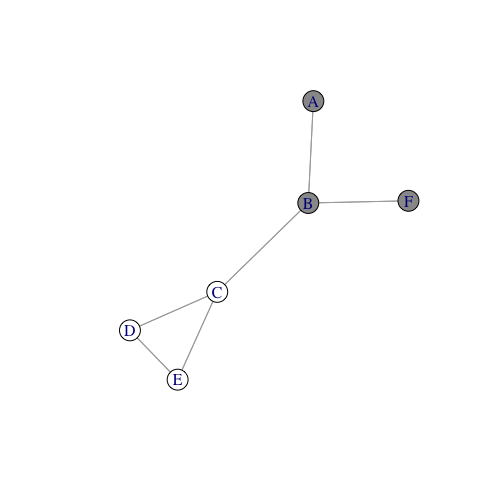
\includegraphics{Network-analysis-/figures/simgraph.png}

\begin{table}
\centering
\caption{Node topology}
\begin{tabular}{lllll}
Node & Node degree & Clustering coefficient & Betweenness   \\
A    & 2           & 0                      & 0             \\
B    & 6           & 0                      & 14            \\
C    & 6           & 0.06                   & 12            \\
D    & 4           & 0.17                   & 0             \\
E    & 4           & 0.17                   & 0             \\
F    & 2           & 0                      & 0            
\end{tabular}
\end{table}

Measures of local properties of networks seek to identify the most important nodes in a network. Different measures indices the different contexts for the word ``importance''. In this study, we consider 3 features of local properties. 

\begin{itemize}

\item \textbf{Node degree} is the number of neighbors of a node, also known as connectivity. Nodes with high degree can be implied that the node has many connections or relationships with other nodes. In co-occurrence network, the high degree node can be inferred that it was found together with occurs with connected nodes. For example, in fig(), node B, and node C are the highest-degree nodes in this network. Node B have the relationships with 3 nodes. We can consider node B as the important node of this network because If we remove this node, there will be two nodes (node A and F) would disappear from this network.

\item \textbf{Local clustering coefficient} is a measure of the degree to which nodes tend to cluster together. It is defined as how often a node forms a triangle with its direct neighbors, proportional to the number of potential triangles the relevant node can form with its direct neighbors. In the context of this network, local clustering coefficients is the the probability that two neighbors of connected with each other in the network. These measures are indicative of the complex forming of co-occurrence patterns through the network. As presented nodes can be observed other nodes, a more closely connected network facilitates nodes co-occurrence. The higher clustering coefficient injury has high possibility to form complex. Node D and E have high clustering coefficient. They formed the complex relationships, which Node D connected with Node E connected to Node C, and Node C also connected with Node D. It indicated that they have close relationships. In the context of co-occurrence network, these three nodes usually occur together.

\item \textbf{Betweenness} is measure the number of paths, which a node is present on the shortest path between all other nodes. Nodes with high betweenness have been shown that there are many pair-wise relationships across a network pass through the node, which is implied that the nodes has high possibility to occur (easily to be induced). We determine high-betweenness injuries as``indicator''. We hypothesize that these indicators, just like hubs, also play central roles in biological networks. 

\end{itemize}

Global properties of the network may also be of interest. They were used to analyze how certain networks contrast to each other. In this study, we measured diameter, global clustering coefficient, average short path to quantify the global properties of networks.  Diameter can be defined as the maximum geodesic distance over the network. Here the network (Fig) we find that this distance is 3, which is from Node A or B to D or E. Global clustering coefficient is defined as the probability that adjacent node of anode connected. For this sample network, it is 0.03 indicating that a few nodes that are connected together. Average short path is measured the average of length of all the shortest paths in the network. The average short path of this network is 1.89. It indicated that the connection between node required at least almost 2 connections in order to reach other nodes. Complexity of networks can infer to the network behavior or the co-occurrence patterns in this study, which is indicated by closeting coefficients and average short path. In high-complex network, nodes are close to each other with many strong connections. Increasing complexity makes network structure tight, and difficult to segregate.   

Moreover, we inspected the community structure of the networks derived from the empirical data to identify the injury symptoms (the combination of injuries) that are especially highly connected based on the optimal clustering algorithm. Such communities correspond to groups of injuries that are closely associated or often formed co-occurrence relationships

\subsubsection{Communities, Structures and compositions of co-occurrence network of rice pest injuries}
\paragraph{Tamil Nadu, India (TMN)}

Dry season network (Fig) was composed of 6 associated injuries (DH, NB, SR, FS, RB, and LF) and captured 7 associations. The network showed two groups of injury syndromes (the combination of injuries). The groups of the injury profiles corresponded to each community based on the optimal clustering algorithm. The first group is composed of DH, LF, RB and SR. Another group consists of FS and NB. Analysis of network properties revealed that LF and FS are high-betweenness nodes. They presented co-occurrence relationships within group 1 and group 2. SR and RB have high clustering coefficient. It indicated that these two injuries usually formed complex of co-occurrence relationships. As opposed to other injuries, NB and DH have low scores on all three centrality measure. Apparently, these injuries less possibly co-occur with other injuries (low betweenness), and do not have complex co-occurrences with other injuries (low degree and clustering coefficient).

Wet season network (Fig) was composed of 12 nodes (injury variables, DP SR, FS, BLB, NB, LF, GLH, RT, RB, DH, WM, BPH) with edges. Fig reveals three groups of injury profiles. DH, GLH, SR and BPH are in the group 1 (green).  FS, NB, DP, BLB is in group 2 (orange). RT, LF, RB and WM are in group 3 (purple). Top four injuries with high betweenness, DP, SR, LF, and BLB, are the members of each of group. They possibly are found co-occurrence within the group and inter-groups of injury profiles. Considered in each group, DH and GLH have high clustering coefficient in the group 1. NB has high clustering coefficient in the group 2. RT has highest clustering coefficient comparing other injuries in the group 3.  Group 2 has high clustering coefficients indicating that this group is closed clustered, and the injuries in this group formed co-occurrence.  DP and SR are important as the linkage to occur with other groups of injuries profiles because of high betweenness and degree. WM, BPH have low value of the 3 local properties. It indicated that BPH and WM were less possible to occur, and present co-occurrence patterns, and when they were observed, they were also not able to relate to many injuries. 

%=========================================
\paragraph{West Java, Indonesia (WJV)}
 
Dry season network (Fig.) composed of 20 nodes and 51 associations. The network reveals four groups of injury profiles. Group 1 (green color) include DH and RT. Group 2 (orange color) is NBS RB, FS, BLS, LB, DP, BLB, NB, BS. Group 3 (purple color) included GM, LF, BPH, SR, SHB, GLH, RS. Group 4 (pink color) include WM and WH.  The second and third group are formed closely clusters.  RT in group 1, BLB and BS in the group 2, LF of group 3, and WM in group 4 are high-betweenness nodes with intermediate clustering coefficient.  NBS, NB, RB, BLS, FS, DP of group 2 have high clustering coefficients. Compared to group 2, the injuries in group 3 have relatively smaller than. It indicated that the injuries in the group 2 are tightly formed complex co-occurrence.  DH, WH have low value of the three features, and located far from the center of the network. BPH and WM were less possible to occur, and present co-occurrence patterns, and when they were observed, they were also not able to relate to many injuries. connectivity.

Wet season network (Fig.) composed of 19 injuries (WM, LF, GLH, DH, BLS, WH, NBS, FS, DP, RS, LB, WPH, SR, SHR, SHB, NB, BS and BLB) with 25 associations. The network was loosely connected (low clustering coefficients). It reveals 3 connected groups and one isolated group of injury profiles. Group 1 (green) DH, WM, SHB, WH, GHL, LF, LB, and RS. Group 2 (orange) is composted of WPH, SR, GM, BLS and DP. Group 3 consisted of FS, NBS, SHB, BLB. Group 4, which is isolated, is composted of BS and NB. In group 1, WM is the injuries with high betweenness, and WH is the injury with high clustering coefficient. In group 2, BLS has high betweenness, and DP has high clustering coefficient. FS in group 3 node with high betweenness and high clustering coefficient. Group 1 appeared to form complex co-occurrence patterns because the average of clustering coefficient of injuries in this group are higher than other groups of injuries.  

%=================================
\paragraph{Central Luzon, Philippines (LAG)}

The dry season network reveal three clustered groups of injury profiles. Group 1 composted of WM, RB, NB, SHB, and FS. WM and RB in this group have high rank of betweenness. Group 2 consist of LB and DP. DP in this group connected with BPH (high betweenness) from group 3, which have GLH, BPH and BLB. Interestingly, SHB in group1, and GLH in group 3 have high clustering coefficients. NB, LB, FS, and BLB featured low in three of centrality. 

Figure revealed co-occurrence network of injury profiles in dry season at Laguna, the Philippines. Network resulted four groups of injury profiles, which there are three connected and one isolated. Group 1 (green) has  SHR, RS, RT, which is isolated. Group 2 (orange) has NB, RB, GLH, BLS, and DP. This group has more more complex combination than others because the clustering coefficients of injuries in this group are higher. Group 3 (purple) has LB, SHB, LB. This group is between group1 and group 4 (pink), which has NBS, LF, BS, and BLB. The position of SHB, LB and WM in the group with high betweenness, but they do not form the the complex combination of the injuries. They tend to link the co-occurrence of the first and the fourth group of injury profiles, which connected to NB in the first group and LF in the fourth group. So they are potentially good target to be monitored too. For example, when LF presented without the present of LB, SHB, WM, it is less likely NB would present, and other injuries in the first group would less likely to present neither. 


\paragraph{Suphan Buri, Thailand (SUP)}

Dry season network shows 8 injuries (DH, BS, SR, SHB, NBS, SHR, GLH, and WH) showing 12 significant relationships. The network revealed three closed cluster of co-occurrence patterns of injuries. Group 1 (green) is composted of NBS, DH, BS, and SHB. Group 2 (orange) is SHB and GLH, and group 3 (purple) is SR and WH. Group 1 is more complex than other two groups because three out of four nodes in the groups presenting high clustering coefficient. NBS, DH, SHB, and SR seem to be clustered together. BS present high betweenness in the first group, which is associated with the other two groups. SHB has high moderate degree and high betweenness, whereas it has low betweenness.  It can form complex association with the injuries in the first group and the second group itself.  WH and GLH feature low scores on at least two centrality measures. Apparently, they are less easily found with other injuries, do not tend to complex combination (low clustering coefficient), or less possible for expressing co-occurrence through the network (low betweenness). 

Network of co-occurrence patterns of injury profiles wet season at Suphan Buri, Thailand revealed 18 associated injuries (DH, BS, SR, SHB, NBS, SHR, GLH, and WH), and 79 associations. Network analysis resulted three closely clustered groups. Group 1 (green) composted of NBS, FS, RT, SHB, LB, WM, RS and RB. Group 2 (orange) consist of GLH, BS, GM, SR, BLB, BLS, LF and DP. Group 3 consisted of SHR and NB. The group 1 are bigger and 3 were relatively high clustering coefficients than other two groups of injuries. RB, NBS, LF, and BS were highly associated in wet season. Even though they were not in the same group, but group 1 and 2 were close, which is indicated by the positions in the network. Interestingly, SHR in group 3 has high betweenness, which is in-between the association of injuries of group 1 and group 3. So SHB is more likely to present in wet season, and form complex association with other injuries because it connected to the high clustering coefficient groups.

\newpage

\paragraph{Makong Rive Delta, Vietnam (MKD)}

Co-occurrence network of injury profiles of dry season in Mekong Rive Delta, Vietnam presented 20 injuries (DH, BS, SR, SHB, NBS, SHR, GLH, and WH) with 61 associations. The network reveals the three groups of injury profiles. The group 1 (green) consisted of LB, DP, RB, DH, BS, and FS. The group 2 (orange) was composed of GLH, WPH, SR, WH, BPH, RS, WM. And the group 3 (purple) consisted of RT, NB, SHB, BLB, LF, and NBS. RB in the group 1 has high rank of betweenness and clustering coefficients. The betweenness of injuries in group 2 ranged low to intermediate, but their clustering coefficients are relatively high. This indicated that they are more likely to form complex association within group than between groups. BLB in group 3 and BS in group 1 have high rank of betweenness and they were associated. The average clustering coefficient of group 1 and 3 are smaller than the group 3. So group 1 and 3 are more likely to have chance to form association between the groups.

Co-occurrence network of injury profiles in wet season at Mekong River delta, Vietnam presented 21 related injuries (DH, BS, SR, SHB, NBS, SHR, GLH, and WH), and 54 associations. From the structure of this network (Fig), it seems to have three clustered groups base on optimal clustering algorithm. The group 1 (green) is composed of NB, SR, BS, WPH, RS, WM, DH, GLH, FS, RT. The second group (orange) has BLB, BPH, LB, NBS, SHB, SHR, DP. The third group is the smallest groups, which has RB, LF and WH. The members within the first groups are relatively close following the layout, and have similar level of clustering coefficients. SHB and RB, RT, LB have high node degree and betweenness, which are inferred that they have possibility to occur in wet season because they shared many co-occurrence patterns with others. Even though, SHB have high level of betweenness and node degree, but intermediate clustering coefficient.  It connected to the high-betweenness injuries such as RB and RT, where are in different groups. SHB also acted like a ``bridge'', which link the injuries of the group 1 and group 2.

\subsubsection{Global properties of the networks}

Complexity of networks indicates the structure of networks, which reflect to the co-occurrence patterns of injury profiles. As shown in Table, we considered the global properties of the two seasonal networks by each location. Dry and wet season networks of WJV, and TMN were similar by considering the value of clustering coefficient, average short path, and diameter. For LAG, MKD, except SUP, clustering coefficient of dry season network are higher and average short path are shorter. Diameter of dry season network also smaller than wet season. Apparently, dry season network are more compact, and present complicated patterns of co-occurrence. 

%table\ref{table:Network_stat}
% Please add the following required packages to your document preamble:
\begin{table}[]
\centering
\begin{tabular}{llllllll}
\hline
\multirow{3}{*}{Country} & \multicolumn{6}{c}{year} & \multirow{3}{*}{Total} \\ \cline{2-7}
                         & \multicolumn{2}{c}{2010} & \multicolumn{2}{c}{2011} & \multicolumn{2}{c}{2012} &                        \\ \cline{2-7}
                         & DS         & WS          & DS          & WS         & DS          & WS         &                        \\
\hline
India                    &            & 25          & 60          &            & 20          &            & 105                    \\
Indonesia                & 5          & 20          & 30          & 30         & 20          &            & 105                    \\
Philippines              &            & 20          & 20          &            &             &            & 40                     \\
Thailand                 &            & 20          &             & 45         &             & 40         & 105                    \\
Vietnam                  &            & 20          &             & 15         & 25          &            & 70                     \\
\hline
Total                    & 5          & 115         & 110         & 90         & 65          & 40         & 425    \\
\hline               
\end{tabular}
\caption{Number of farmers' fields surveyed by country and year}
\label{table:Survey_data}
\end{table}
\begin{table}
\centering
\caption{rice production season}
\label{table:rice-production-season}
\begin{tabular}{lllll}
\multicolumn{1}{c}{\multirow{2}{*}{Country}} & \multicolumn{2}{c}{Dry}                                       & \multicolumn{2}{c}{Wet/Winter*}                            \\
\multicolumn{1}{c}{}                         & \multicolumn{1}{c}{Planting} & \multicolumn{1}{c}{Harvesting} & \multicolumn{1}{c}{Planting} & \multicolumn{1}{c}{Harvest} \\
Indonesia                                    & April                        & October                        & November                     & March                       \\
India                                        & November                     & Mar                            & Jun                          & October                     \\
Philipppines                                 & November                     & April                          & May                          & Octber                      \\
Thailand                                     & January                      & June                           & August                       & December                    \\
Vietnam                                      & December                     & April                          & April                        & August                     
\end{tabular}
\end{table}
\begin{table} 
    \begin{tabular}{ c c c c c c c c c c c }
    \hline
         Country & Node & Link & Diameter & Connectivity & Geodesic & Density & Smallworldness & Centrality & Heterogeneity \\ 
         \hline
         India & 10 & 17 & 1.38 & 0.55 & 2.02 & 0.14 & 1.71 & 0.14 & 0.51 \\
         Indonesia & 22 & 48 & 1.40 & 0.46 & 2.25 & 0.06 & 1.24 & 0.07 & 0.64 \\
         Philippines & 21 & 33 & 1.85 & 0.28 & 2.26 & 0.07 & 0.82 & 0.19 & 0.89 \\
         Thailand & 18 & 63 & 1.11 & 0.47 & 1.81 & 0.15 & 1.07 & 0.20 & 0.70 \\
         Vietnam & 20 & 47 & 1.24 & 0.53 & 2.05 & 0.08 & 1.27 & 0.08 & 0.47 \\ 
     \hline  
    \end{tabular} 
    \caption{Network statistics for network graph each country}
\label{table:Network_stat}
\end{table}


%=== Here is the temp files
